Khối đa hợp địa chỉ (Address Mux) là một mạch tổ hợp lựa chọn địa chỉ đi vào bộ nhớ (Memory) dựa theo chu kì hoạt động. 
Ngoài ra khối còn được thiết kế với tham số \textbf{width} (mặc định 32-bit), cho phép dễ dàng mở rộng không gian địa chỉ khi cần thiết.

\begin{figure}[H]
    \centering
    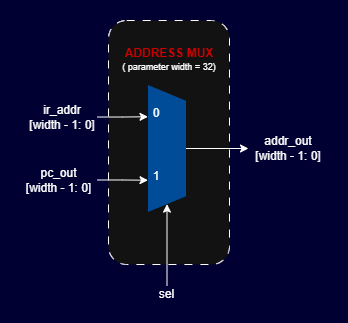
\includegraphics[width=0.7\textwidth]{Address_mux.png} 
    \caption{Sơ đồ khối bộ đa hợp địa chỉ (Address Mux)}
    \label{fig:address_mux}
\end{figure}

\textbf{Nguyên lý hoạt động:}
Khối Address Mux hoạt động dựa vào tín hiệu \textit{sel} từ khối Controller với logic hoạt động như sau:

\begin{itemize}
    \item \textbf{Giai đoạn nạp lệnh ($sel = 1$):} 
    \texttt{Address Mux} sẽ ưu tiên lựa chọn địa chỉ từ \texttt{PC} ($pc\_out$). 
    Lúc này địa chỉ của lệnh tiếp theo sẽ được đưa đến bộ nhớ để thực hiện quá trình lấy lệnh (Instruction Fetch).
    
    \item \textbf{Giai đoạn thực thi ($sel = 0$):} 
    \texttt{Address Mux} chuyển sang lựa chọn địa chỉ toán hạng từ \texttt{IR} ($ir\_addr$). 
    Việc này giúp CPU định vị được vị trí toán hạng để đưa vào tính toán.
\end{itemize}